\section{Introduction}\label{sec:introduction}

This document presents a template for writing reports.

A citation looks like this: \cite{10285163}

\subsection{Figures}\label{subsec:figures}

\begin{figure}
    \centering
    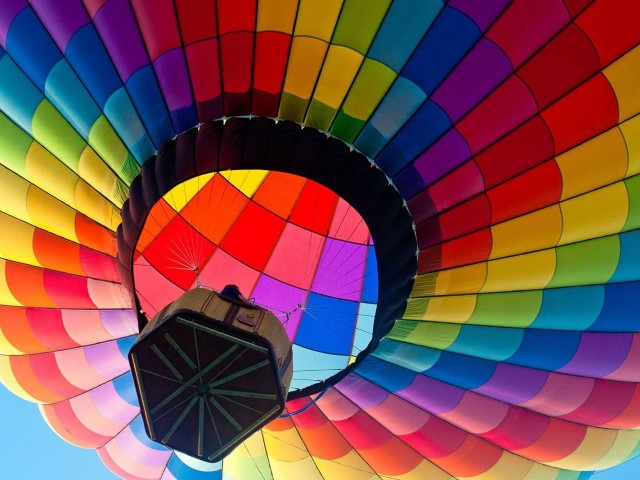
\includegraphics[width=0.4\linewidth,height=\textheight,keepaspectratio]{images/hot-air-balloon.jpg}
    \caption{A hot air balloon}\label{fig:logo}
\end{figure}

In Figure~\ref{fig:logo} we can see..


\subsection{Circuits}\label{subsec:circuits}

\begin{figure}
\centering

\begin{circuitikz}
\draw (0,0) node (start) {}
to[sV=$V_i$] ++(0,2+\ctikzvalof{tubes/height})
to[C=$C_i$] ++(2,0) coordinate(Rg)
to[R=$R_g$] (Rg |- start)
(Rg) to[short,*-] ++(1,0)
node[triode,anchor=control] (Tri) {} ++(2,0)
(Tri.cathode) to[R=$R_c$,-*] (Tri.cathode |- start)
(Tri.anode) to [R=$R_a$] ++(0,2)
to [short] ++(3.5,0) node(Vatop) {}
to [V<=$V_a$] (Vatop |- start)
to [short] (start)
(Tri.anode) ++(0,0.2) to[C=$C_o$,*-o] ++(2,0)
(Tri.cathode) ++(0,-0.2) to[short,*-] ++(1.5,0) node(Cctop) {}
to[C=$C_c$,-*] (start -| Cctop)
;
\draw[red,thin,dashed] (Tri.north west) rectangle (Tri.south east);
\draw (Tri.east) node[right] {12AX7};
\end{circuitikz}

\caption{Triode amplifier}\label{fig:triode_amplifier}
\end{figure}


\subsection{Code}\label{subsec:code}

\begin{lstlisting}[language=Python, caption={The preprocessing step}, label=lst:python]
    def set_custom_lmclks():
        """Populate LMK and LMX clocks. Search for clock files.
        Obtain the properties of the clock files. Program the
        LMK and LMX clocks with the properties of the files.
        """
        
        # Ensure LMK and LMX devices are known
        _get_lmclk_devices()
        
        # Get custom ref clock locs
        cwd = os.path.dirname(os.path.realpath(__file__))
        lmk_loc, lmx_loc = _get_custom_lmclks(cwd)
        
        # Get custom ref clock props
        clk_props = _get_custom_lmclk_props(lmk_loc, lmx_loc)
        
        # Program custom ref clocks
        _program_custom_lmclks(clk_props)
\end{lstlisting}

A code listing can be found in Listing~\ref{lst:python}.
